\begin{justify}
Dans cette section, nous présentons les principales interfaces développées durant cette sprint 2.2, en commençant par celles liées à l'exécution parallèle des tests, la gestion des rapports, puis la visualisation des statistiques.
\end{justify}
\begin{itemize}[label=$\bullet$]
    \item \textbf{Interface de la sélection des tests à exécuter} :  
    La figure \ref{fig:multiScanUI}\footnote{Voir annexe E : Figure \ref{fig:multiScanUI}} illustre l’interface permettant à l’utilisateur de sélectionner un ou plusieurs types d’analyses à effectuer (fonctionnelle, sécurité, SEO). Cette interface a été conçue pour offrir une interaction simple et efficace, favorisant l’exécution parallèle des différents scans.

    \item \textbf{Interface de visualisation consolidée des résultats} :  
    La figure \ref{fig:resultView}\footnote{Voir annexe E : Figure \ref{fig:resultView}} présente la vue unifiée des résultats d’analyse. Elle regroupe les vulnérabilités de sécurité, les erreurs fonctionnelles et les recommandations SEO dans une seule interface pour faciliter la lecture croisée et la prise de décision.

    \item \textbf{Interface de gestion des rapports d’analyse} :  
    Comme illustré dans la figure \ref{fig:reportManagementUI}, cette interface permet à l’administrateur de rechercher, supprimer, exporter les rapports. Les filtres intégrés (type, date, utilisateur) rendent la gestion des rapports plus fluide et performante.
    \begin{figure}
        \centering
        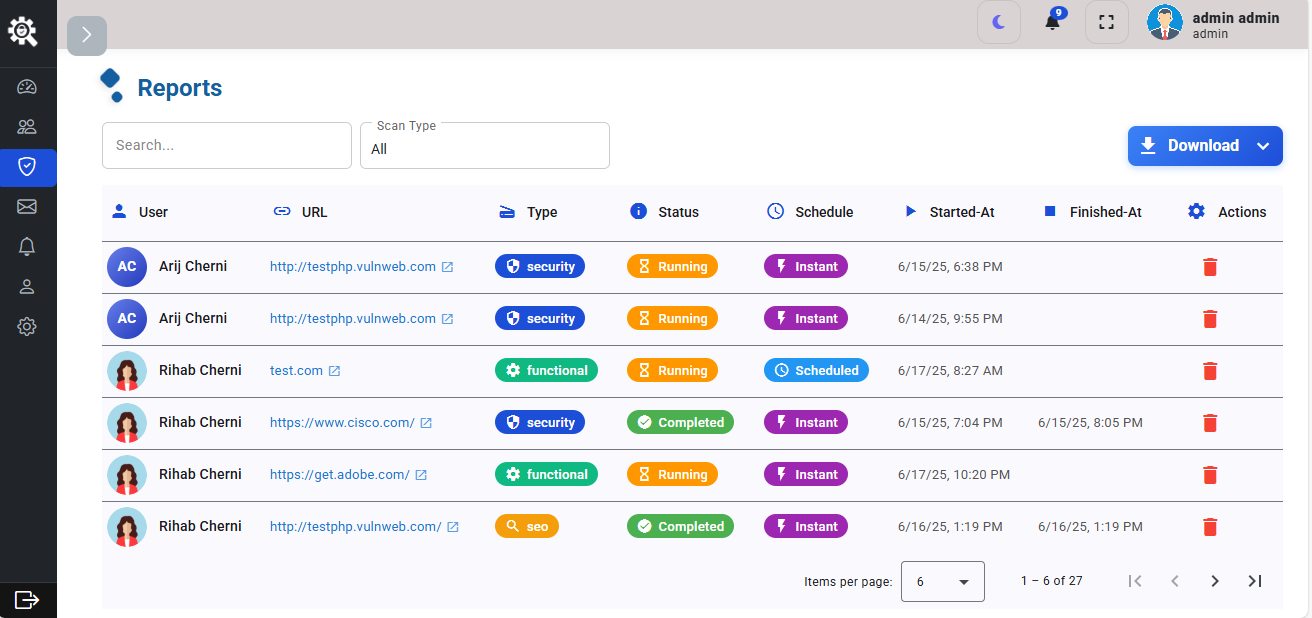
\includegraphics[width=\linewidth]{chapitres/ch4Sp2/section/sprint2.2/img/interface/reports-admin-liste.PNG}
        \caption{Caption}
        \label{fig:enter-label}
    \end{figure}

   \item \textbf{Tableau de bord utilisateur} :   La figure \ref{fig:testerdashboardUI}présente le tableau de bord dédié aux testeurs. Il affiche  des statistiques filtrables et interactives sur les campagnes de test, à travers des graphiques dynamiques.
    \begin{figure}[H]
        \centering
        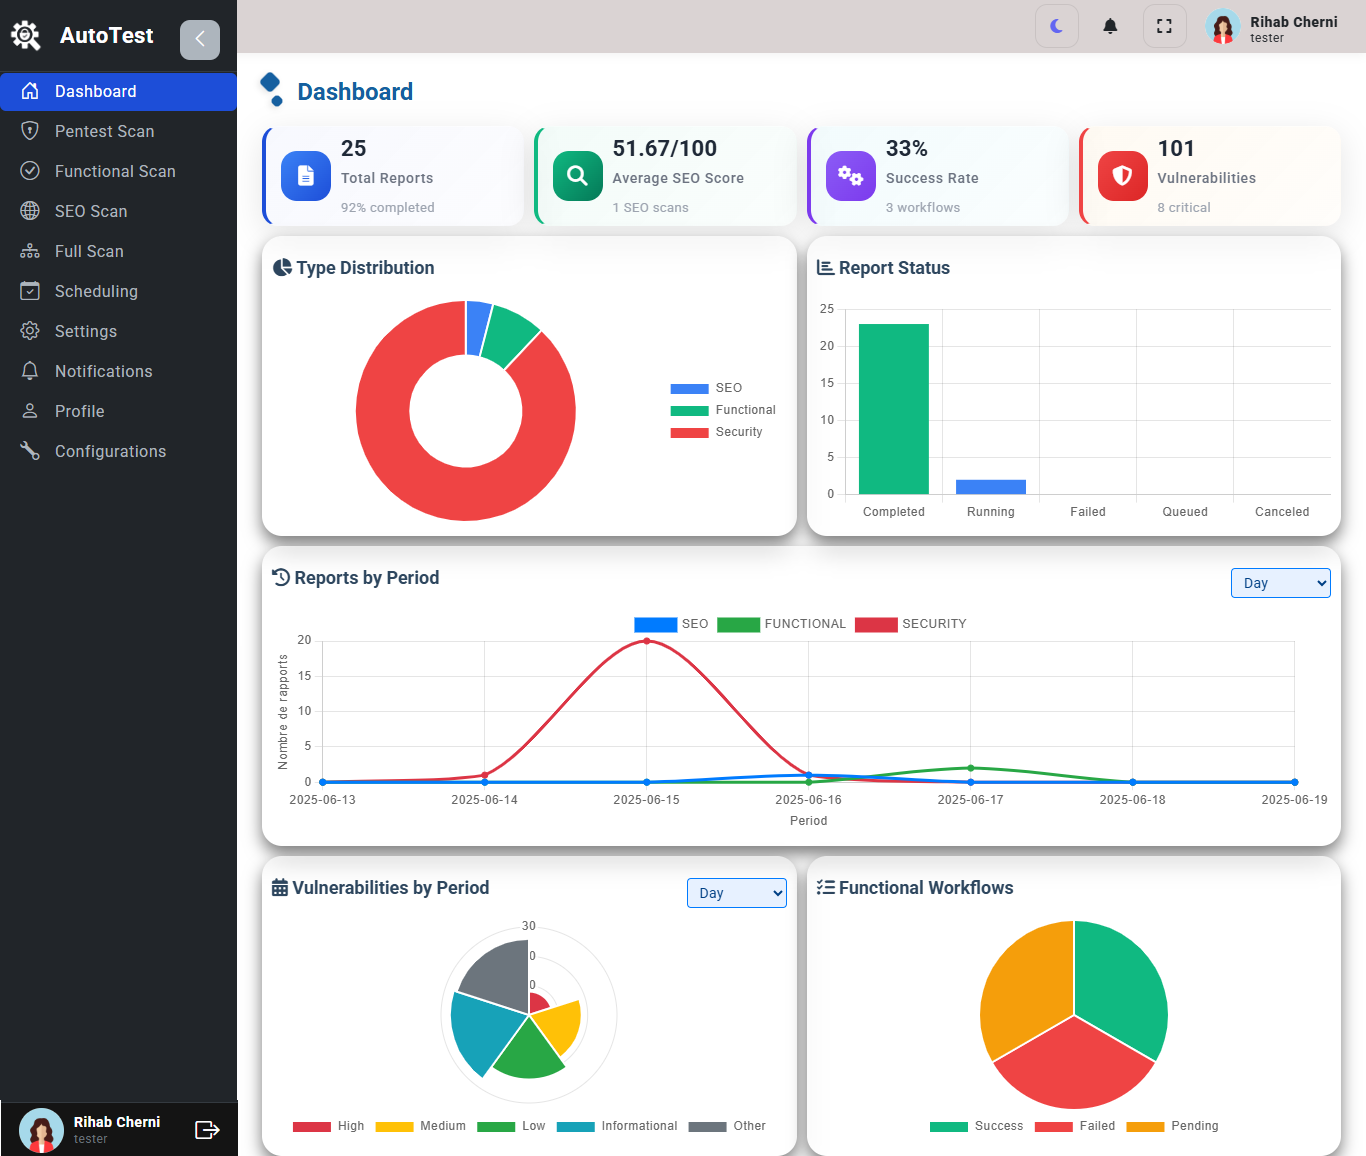
\includegraphics[width=\linewidth]{chapitres/ch4Sp2/section/sprint2.2/img/interface/tester-dashbaord.png}
        \caption{\centering Interface du tableau de bord testeur}
        \label{fig:testerdashboardUI}
    \end{figure}
    \vspace{-0.3cm}
    \item \textbf{Tableau de bord administrateur} :  
    Pour le profil administrateur, la figure \ref{fig:adminDashboardUI} met en évidence les indicateurs globaux sur l'activité de la plateforme : nombre de scans, utilisateurs actifs, types d’analyses effectuées, etc. Des filtres par période ou type d’analyse sont également disponibles.
    \begin{figure}[H]
        \centering
        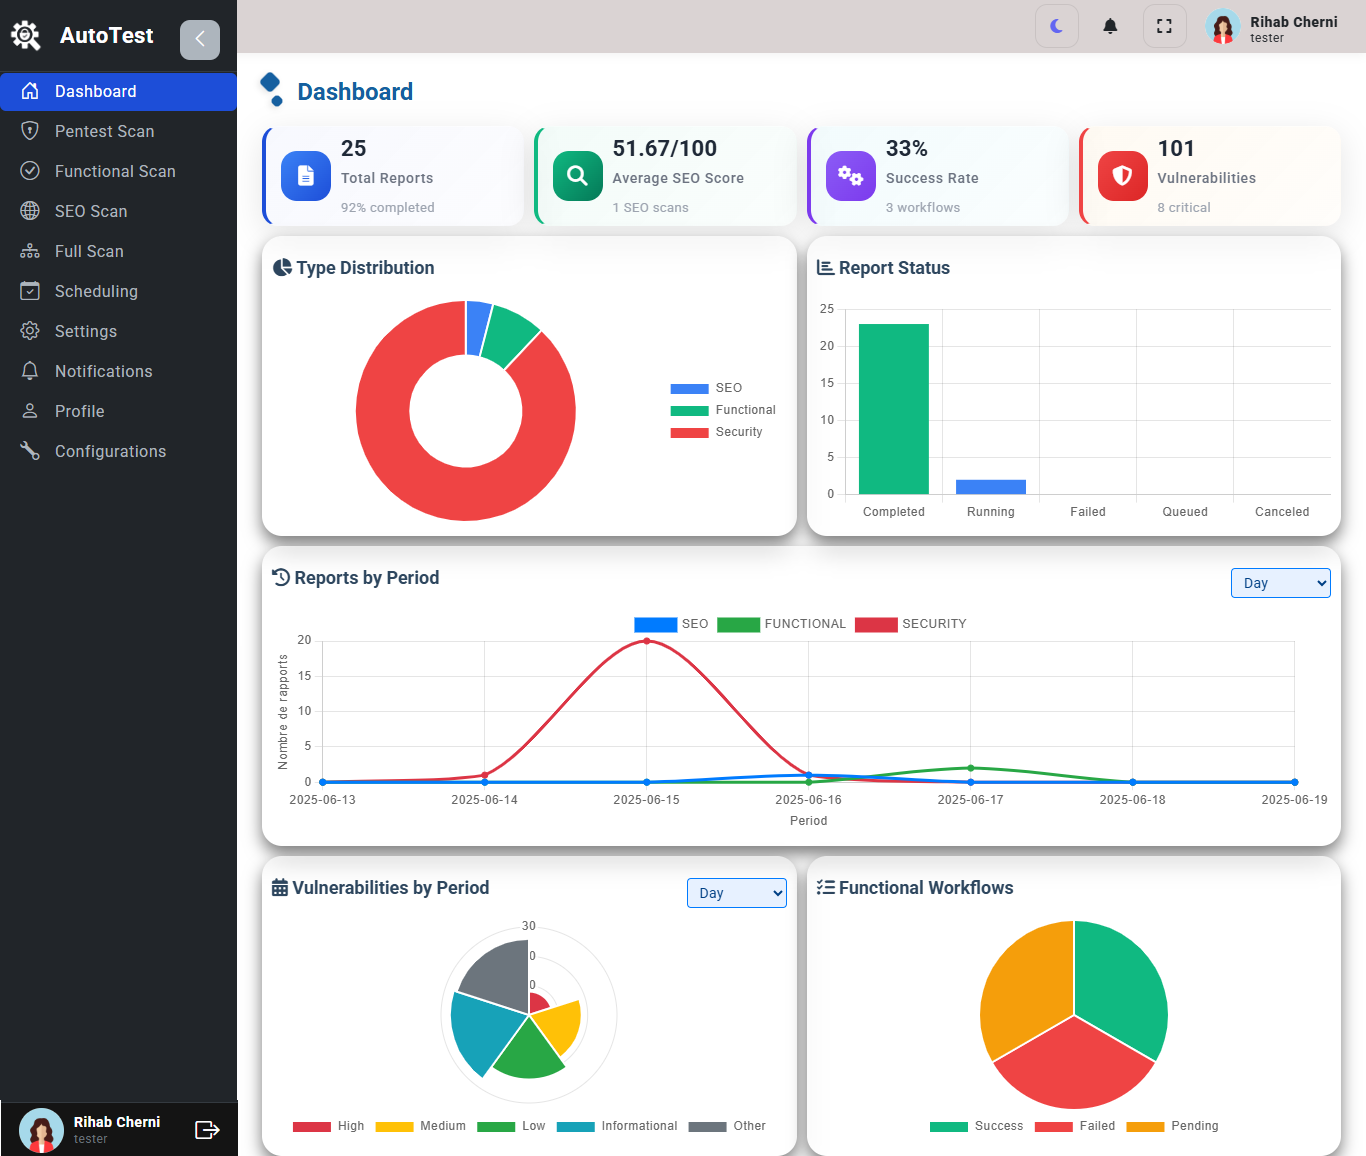
\includegraphics[width=\linewidth]{chapitres/ch4Sp2/section/sprint2.2/img/interface/tester-dashbaord.png}
        \caption{\centering Interface du tableau de bord testeur}
        \label{fig:testerdashboardUI}
    \end{figure}
    \vspace{-0.3cm}

    \item \textbf{Déploiement par conteneurisation} :  
    La figure \ref{fig:deploymentInterfaceUI}\footnote{Voir annexe E : Figure \ref{fig:deploymentInterfaceUI}} illustre le tableau de gestion du déploiement via Docker. Cette interface permet de visualiser le statut de chaque conteneur (backend, frontend, outils de scan), avec la possibilité de redémarrer individuellement les services.
\end{itemize}
